% ======================================================================
% CNF / NFVI Testbed — Project III (IT3943)
% Tô Hùng Anh — MSSV 20225164 — HUST
% ======================================================================
\documentclass[12pt]{article}

\usepackage[utf8]{inputenc}
\usepackage[english]{babel}

\usepackage[export]{adjustbox}
\usepackage{amsmath}
\usepackage{amssymb}
\usepackage{anysize}
    \marginsize{2cm}{2cm}{2cm}{2cm}
\usepackage{appendix}
\usepackage{caption}
    \captionsetup{labelfont={bf}}
\usepackage{cite}
\usepackage{color}
\usepackage{fancyhdr}
    \pagestyle{fancy}
    \fancyhf{}
    \fancyfoot[C]{\thepage}
    \renewcommand{\footrulewidth}{0.4pt}
\usepackage{float}
\usepackage{graphicx}
\usepackage{indentfirst}
\usepackage{siunitx}
\usepackage{subcaption}
\usepackage{titlesec}
    \titleformat{\section}{\Large\bfseries}{\thesection}{1em}{}
    \titleformat{\subsection}{\large\bfseries}{\thesubsection}{1em}{}
    \titleformat{\subsubsection}{\normalsize\bfseries}{\thesubsubsection}{1em}{}
\usepackage{booktabs}
\usepackage{listings}
\usepackage{xcolor}

\newcommand{\HRule}{\rule{\linewidth}{0.5mm}}
\renewcommand{\appendixpagename}{\LARGE Appendices}

% Colors
\definecolor{istblue}{RGB}{3, 171, 230}
\definecolor{dkgreen}{rgb}{0,0.6,0}
\definecolor{codebackground}{RGB}{248, 248, 248}
\definecolor{codeborder}{RGB}{220, 220, 220}
\definecolor{keywordcolor}{RGB}{0, 0, 255}
\definecolor{stringcolor}{RGB}{163, 21, 21}
\definecolor{commentcolor}{RGB}{0, 128, 0}
\definecolor{numbercolor}{RGB}{128, 128, 128}

% YAML language definition for listings
\lstdefinelanguage{yaml}{
  keywords={true,false,null,y,n},
  keywordstyle=\color{keywordcolor}\bfseries,
  basicstyle=\ttfamily\footnotesize,
  sensitive=false,
  comment=[l]{\#},
  commentstyle=\itshape\color{commentcolor},
  stringstyle=\color{stringcolor},
  moredelim=[l][\color{dkgreen}]{\&},
  moredelim=[l][\color{magenta}]{*},
  morestring=[b]',
  morestring=[b]"
}

\lstset{
    basicstyle=\ttfamily\footnotesize,
    breaklines=true,
    frame=shadowbox,
    rulesepcolor=\color{codeborder},
    backgroundcolor=\color{codebackground},
    numbers=left,
    numberstyle=\tiny\color{numbercolor}\ttfamily,
    numbersep=10pt,
    keywordstyle=\bfseries\color{keywordcolor},
    commentstyle=\itshape\color{commentcolor},
    stringstyle=\color{stringcolor},
    showstringspaces=false,
    captionpos=b,
    tabsize=2,
    xleftmargin=15pt,
    xrightmargin=5pt,
    framexleftmargin=10pt,
    aboveskip=15pt,
    belowskip=15pt,
}

\usepackage[colorlinks=true, plainpages=true, linkcolor=istblue, urlcolor=istblue, citecolor=istblue, anchorcolor=istblue]{hyperref}

\title{\textbf{A Mini NFVI Platform for Cloud-Native 5G Core Functions: Deploying and Validating Open5GS on Kubernetes (k3s)}}
\author{Hung Anh To \\ \texttt{github.com/hunganh1310} \\ \small IT3943 - Project III \\ \small Hanoi University of Science and Technology}
\date{\today}

\begin{document}

% ----------------------------------------------------------------------
% Cover
% ----------------------------------------------------------------------
\begin{center}
    \textsc{\large \bf Hanoi University of Science and Technology}\\
    \textsc{\large \bf School of Information Technology and Communication}\\[1cm]

    \begin{figure}[H]
        \centering
        
\includegraphics[scale=0.2, center]{Images/hust_logo.jpg}\\[0.8cm]
    \end{figure}

    \textsc{\LARGE REPORT: PROJECT III}\\[0.5cm]
    \HRule\\[0.4cm]
    {\large \bf A Mini NFVI Platform for Cloud-Native 5G Core Functions:\\Deploying and Validating Open5GS on Kubernetes (k3s)\\[0.2cm]}
    \large An NFV Infrastructure that hosts a real containerised 5G Standalone core
    \HRule\\[1cm]
\end{center}

\begin{flushleft}
    \large \textbf{Prepared by:}
\end{flushleft}
\begin{center}
    \begin{minipage}{0.5\textwidth}
        \begin{flushleft}
            \large Tô Hùng Anh
        \end{flushleft}
    \end{minipage}%
    \begin{minipage}{0.5\textwidth}
        \begin{flushright}
            \texttt{\large MSSV: 20225164}
        \end{flushright}
    \end{minipage}\\[0.2cm]
\end{center}

\begin{center}
    \textsc{}\\[2cm]
    \large \bf Ha Noi - 2025
\end{center}

\thispagestyle{empty}
\maketitle
\setcounter{page}{0}

\newpage
\begin{abstract}
\large
The 5G Standalone (SA) core network is no longer a set of specialised
hardware appliances: its functions --- the User Plane Function (UPF), the
Access and Mobility Management Function (AMF), the Session Management
Function (SMF), and others --- are now \textbf{Cloud-Native Network
Functions (CNFs)}: containers orchestrated by Kubernetes. Running them,
however, requires more than a plain Kubernetes cluster. A telco-grade
\textbf{NFV Infrastructure (NFVI)} must provide a dedicated user-plane data
path with multiple network interfaces per pod, elastic scaling of stateless
control functions, and end-to-end observability --- none of which vanilla
Kubernetes offers by default.
\par
This project \emph{designs, builds, and validates} such an NFVI platform on a
single 16~GB laptop, and then \emph{proves it works by running a real 5G core
on it}. A three-node \textbf{k3s} cluster is provisioned entirely through
Infrastructure-as-Code (Vagrant + Ansible). A secondary CNI
(\textbf{Multus + macvlan + Whereabouts}) gives the UPF the separate
N3/N6 user-plane interfaces it needs, kept strictly isolated from management
and cluster-signalling traffic. The open-source \textbf{Open5GS} 5G SA core is
deployed as a set of CNFs, and \textbf{UERANSIM} simulates a gNodeB and a
subscriber. We then demonstrate, end to end, that a UE registers with the
core, establishes a PDU session, and exchanges real user-plane traffic that
traverses the UPF --- alongside autoscaling of stateless network functions and
a Prometheus/Grafana view of the running core. The report makes explicit, at
every step, \emph{why} each platform capability exists by tracing it back to a
concrete requirement of the 5G core it serves.
\end{abstract}

\newpage
\tableofcontents
\newpage

\section{Introduction}

\subsection{Motivation and Background}

The telecommunications industry is undergoing a fundamental shift from
purpose-built, vertically integrated network appliances towards software
running on commodity computing infrastructure. This transformation,
formalised by ETSI as \textbf{Network Functions Virtualisation (NFV)},
decouples network functions (firewalls, routers, load balancers, packet
gateways, etc.) from the proprietary hardware on which they traditionally
ran \cite{etsi002}. In parallel, \textbf{Software-Defined Networking (SDN)}
separates the network control plane from the data plane, enabling
centralised, programmable network management.

The first generation of NFV deployments virtualised network functions as
Virtual Machines (VMs), managed by OpenStack as the Virtual Infrastructure
Manager (VIM). More recently the industry has embraced \textbf{cloud-native}
principles: network functions are packaged as containers and orchestrated by
Kubernetes, giving rise to \textbf{Cloud-Native Network Functions (CNFs)}
\cite{etsi022,lfn}. CNFs boot in seconds, consume far fewer resources, and
inherit Kubernetes' self-healing and horizontal scaling capabilities.

\subsection{Problem Statement}

Production NFV platforms are large, expensive, and operationally complex,
which makes them impractical for learning and experimentation. This project
addresses the question: \emph{can the essential structure and behaviour of
the ETSI NFV framework be reproduced faithfully on a single personal
computer?} The challenge is to build a self-contained testbed that
(i)~maps cleanly onto the ETSI reference architecture, (ii)~exhibits the
telco-grade separation of management, control, and user planes, and
(iii)~fits within a hard budget of 16~GB of host RAM.

\subsection{Objectives}

\begin{enumerate}
    \item Provision a multi-node Kubernetes cluster entirely through
          Infrastructure-as-Code (Vagrant~+~Ansible).
    \item Deploy a CNF with \textbf{multi-NIC} networking that separates
          management, cluster, and data-plane traffic.
    \item Reproduce the telco three-plane network model using a secondary
          CNI (Multus~+~macvlan~+~Whereabouts).
    \item Provide full observability with Prometheus and Grafana.
    \item Demonstrate horizontal auto-scaling (HPA) and measure real
          data-plane throughput.
    \item Establish an explicit mapping between each ETSI NFV building block
          and its Kubernetes equivalent.
\end{enumerate}

\subsection{Report Organisation}

Section~2 reviews the theoretical background (NFV, SDN, OpenStack, and
Kubernetes as a cloud-native VIM). Section~3 discusses the migration from
VM-based VNFs to CNFs and the multi-NIC networking model. Section~4 presents
the system architecture. Section~5 details the implementation. Section~6
reports the testing and evaluation across five test cases. Section~7
concludes and outlines future work.

\section{Background}

This section gives a reader unfamiliar with the field exactly the concepts
needed to follow the rest of the report: the ETSI NFV framework (what an NFVI
is), and the 5G core as a set of cloud-native functions (what runs \emph{on}
the NFVI). We deliberately keep it short and concrete --- only what the design
later depends on.

\subsection{The ETSI NFV framework: who provides, who consumes}

ETSI's reference architecture \cite{etsi002} separates the system into three
domains, shown in Figure~\ref{fig:etsi}.

\begin{figure}[H]
    \centering
    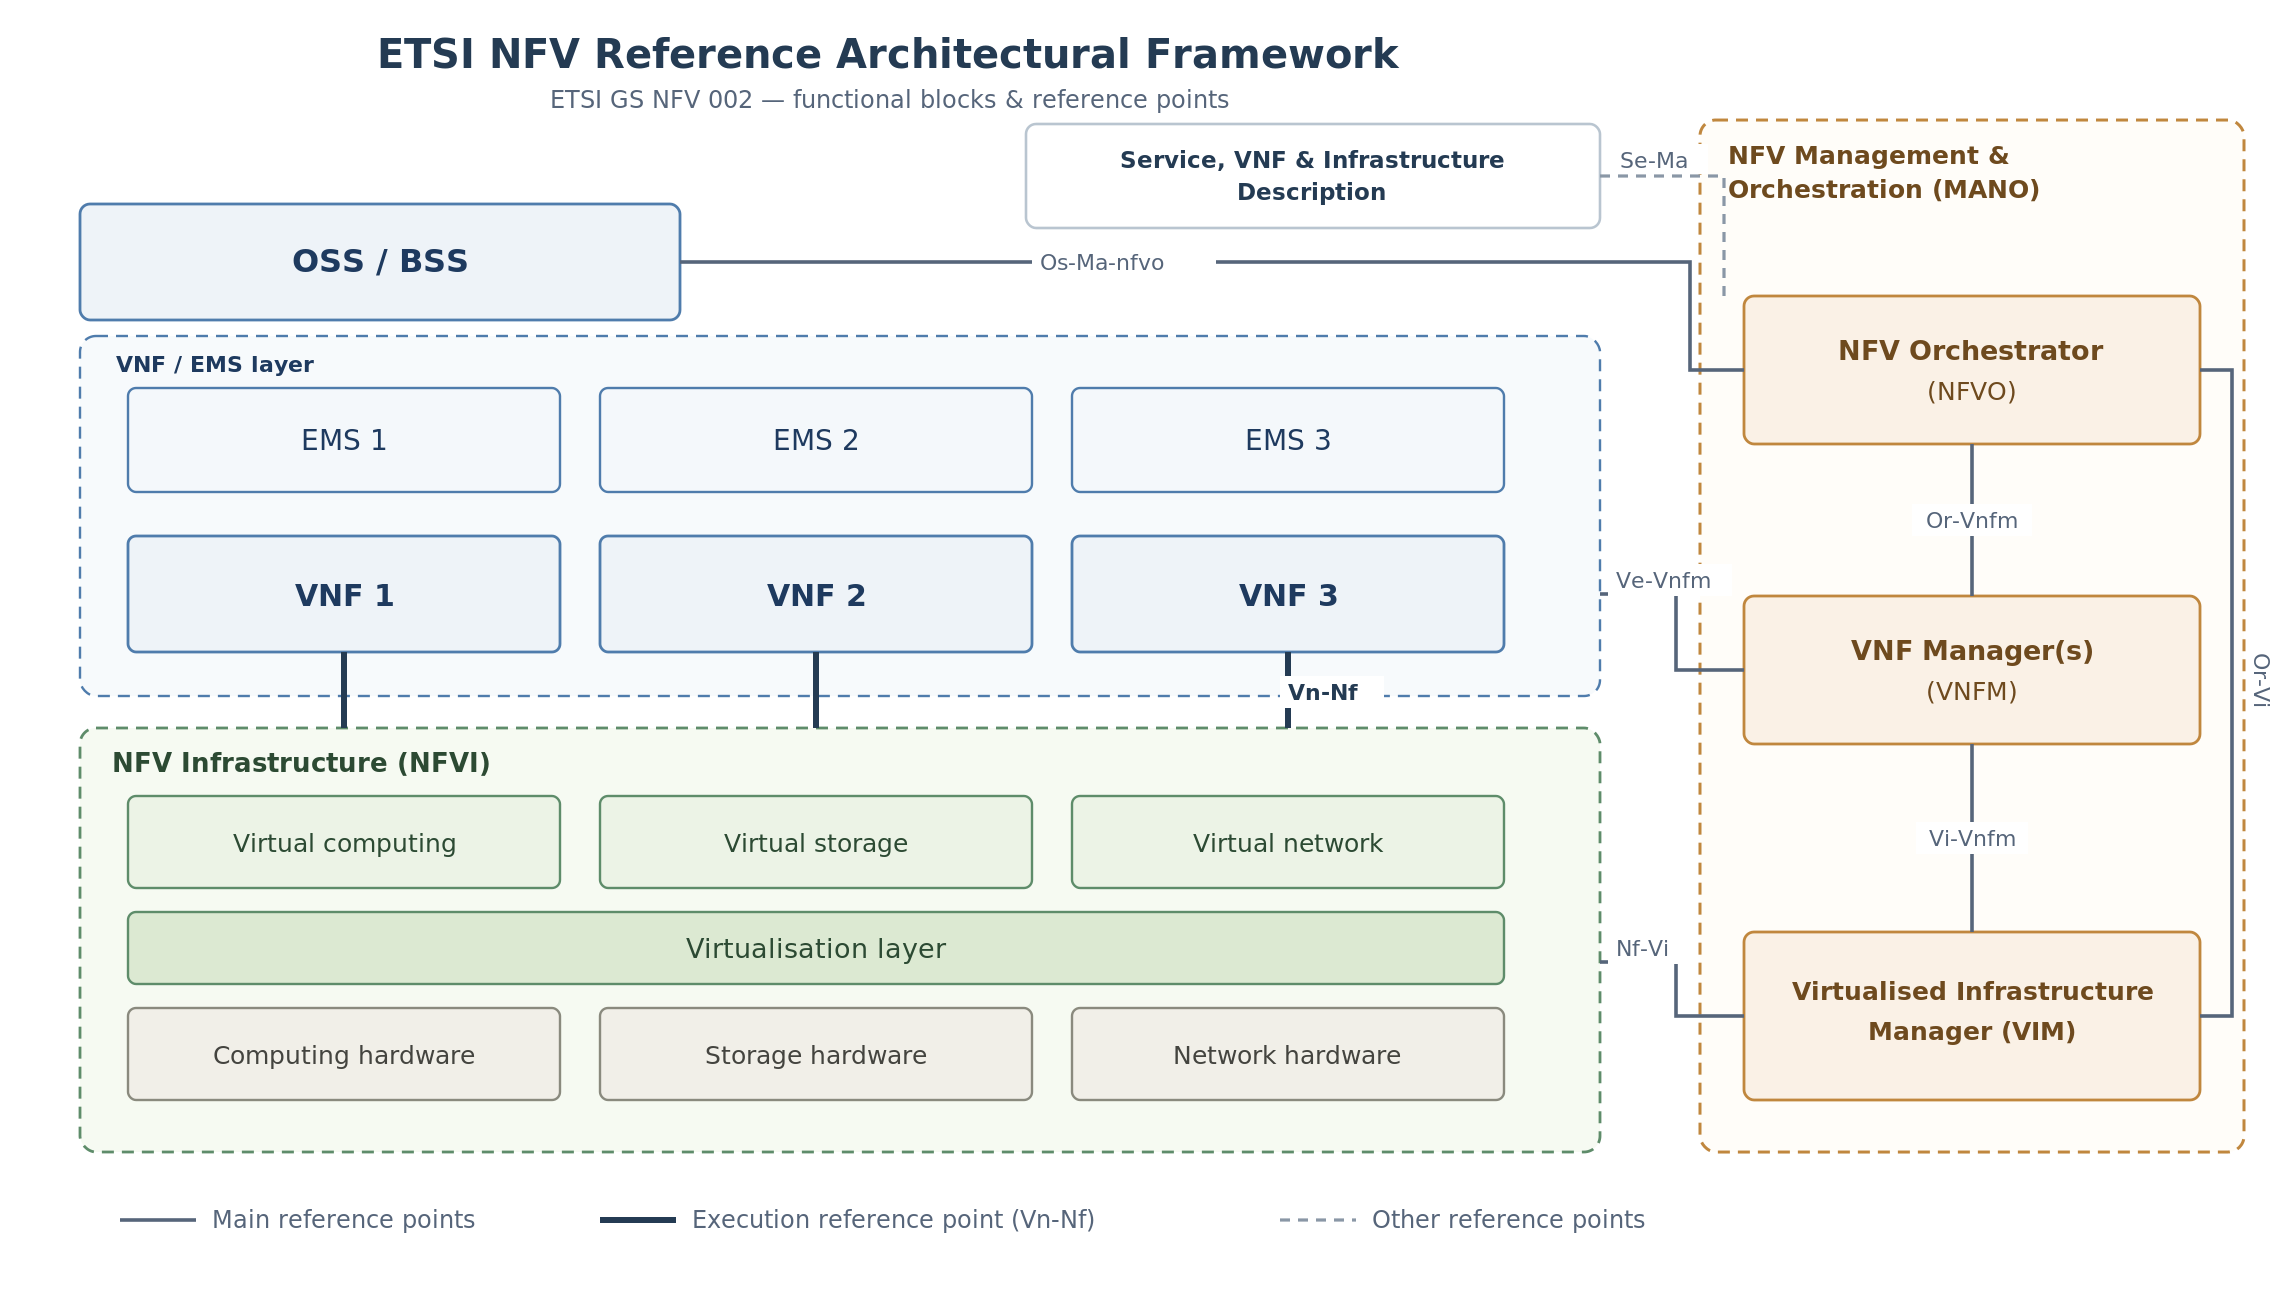
\includegraphics[width=0.9\textwidth]{Images/etsi_nfv_arch.png}
    \caption{ETSI NFV framework and how this project realises each block.}
    \label{fig:etsi}
\end{figure}

\begin{itemize}
    \item \textbf{NFVI} --- the infrastructure: compute, storage, and network,
          plus the virtualisation layer. It is the \emph{provider} of
          resources. In this project the NFVI is the three-node k3s cluster.
    \item \textbf{VNF / CNF} --- the network functions themselves, the
          \emph{consumers} of the infrastructure. Here they are the Open5GS 5G
          core functions, running as containers.
    \item \textbf{MANO} (Management and Orchestration) --- the \textbf{VIM}
          manages NFVI resources (this is Kubernetes/k3s), the \textbf{VNFM}
          manages the lifecycle of each function (here, Helm), and the
          \textbf{NFVO} orchestrates end-to-end network services.
\end{itemize}

The single most important idea is the provider/consumer split: \emph{this
project builds the provider (NFVI) and validates it with a real consumer (the
5G core).} That distinction is what was missing from a naive reading of ``a
three-node cluster''.

\subsection{The 5G Standalone core as cloud-native functions}

The 5G SA core \cite{ts23501} is decomposed into NFs that talk to each other
over a \textbf{Service-Based Interface (SBI)} --- HTTP/2 REST APIs --- much
like microservices. The functions relevant to this project are:

\begin{itemize}
    \item \textbf{AMF} --- handles UE registration and mobility; it is the
          control-plane entry point from the radio network (interface
          \textbf{N2}).
    \item \textbf{SMF} --- manages PDU sessions (a UE's data connection) and
          controls the UPF over interface \textbf{N4}.
    \item \textbf{UPF} --- the \emph{only} user-plane function: it forwards
          actual subscriber packets. It receives them from the radio side over
          \textbf{N3} (a GTP-U tunnel) and sends them to the data network over
          \textbf{N6}.
    \item \textbf{NRF} --- a registry where every NF registers and discovers
          the others; stateless and read-heavy.
    \item \textbf{AUSF, UDM, UDR, PCF, NSSF, SCP} --- supporting control-plane
          functions (authentication, subscriber data, policy, slice selection,
          and an SBI proxy). UDR keeps subscriber records in a database
          (MongoDB).
\end{itemize}

\paragraph{Control plane vs.\ user plane --- the decisive separation.}
5G makes a hard split between the \textbf{control plane} (signalling: who is
this subscriber, may they connect, set up a session) and the \textbf{user
plane} (the subscriber's actual data packets). The control NFs (AMF, SMF, NRF,
\ldots) exchange small SBI messages; the UPF moves bulk traffic at high rate.
This is why the UPF is given its own dedicated network interfaces (N3/N6) and
why, in our cluster, those interfaces must \emph{not} share the path used for
ordinary control signalling. This requirement drives the entire network design
in Section~4.

\subsection{Why Kubernetes alone is not enough}

Kubernetes is an excellent VIM, but a default pod has exactly one network
interface, attached by a single \textbf{CNI} (Container Network Interface)
plugin to one cluster-wide overlay. That suffices for web microservices, but
not for a UPF that needs separate user-plane interfaces. The gap is filled by
a \textbf{secondary CNI}: \textbf{Multus}, a meta-plugin that lets a pod be
attached to additional networks. Section~3 turns this and the other gaps into
an explicit list of requirements.

We use \textbf{k3s} \cite{k3s}, a CNCF-certified single-binary Kubernetes
distribution that replaces etcd with a lightweight embedded datastore --- ideal
for a 16~GB host while remaining fully API-compatible with upstream Kubernetes.

\section{From VNF to CNF: what the platform must provide}

Section~2 introduced the 5G core. This section does the work the original
framing was missing: it derives, from the concrete needs of that core,
\emph{exactly} which capabilities the NFVI platform must offer --- and then
maps each capability onto a specific Kubernetes mechanism. Every design choice
in Sections~4 and~5 traces back to a row of Table~\ref{tab:requirements}.

\subsection{Why containers (CNFs) and not VMs (VNFs)}

The first NFV deployments ran network functions as virtual machines (VNFs) on
OpenStack. That worked, but each VM carries a full guest OS: boot times of
tens of seconds, hundreds of megabytes to gigabytes of RAM before the function
even starts, and multi-gigabyte images. For a 5G core that must scale quickly
with demand, this is too heavy. A \textbf{CNF} re-packages the same function as
containers: it starts in seconds, shares the host kernel, ships as a compact
image, and --- most importantly --- delegates its lifecycle (restart, scale,
heal) to Kubernetes controllers instead of bespoke automation. Open5GS ships
each NF as such a container, which is why the whole core fits on a 16~GB host.

\subsection{Requirements derived from the 5G core}

Table~\ref{tab:requirements} is the heart of the report's argument. The
left column is a concrete fact about the 5G core; the middle column is the
platform capability it forces; the right column is how we provide it.

\begin{table}[H]
\centering
\small
\begin{tabular}{p{0.34\textwidth} p{0.30\textwidth} p{0.28\textwidth}}
\toprule
\textbf{Need of the 5G core} & \textbf{Required platform capability} & \textbf{Provided by} \\
\midrule
UPF forwards user data over dedicated N3/N6 interfaces, separate from signalling
  & A pod must have \emph{multiple} NICs on \emph{isolated} L2 networks
  & Multus + macvlan + Whereabouts (Sec.~4.2, 5.3) \\
Control NFs (NRF, AUSF\ldots) are stateless and scale with signalling load
  & On-demand horizontal scaling
  & HorizontalPodAutoscaler + metrics-server (Sec.~5.4) \\
NFs are independent functions with their own lifecycle
  & Declarative deploy / upgrade / heal per function
  & Kubernetes Deployments + Helm (Sec.~5.4) \\
NFs discover each other over SBI (HTTP/2)
  & Stable virtual IPs and L4 load balancing
  & Kubernetes Service (ClusterIP) \\
An operator must see the core's health and the UPF's load
  & Cluster-wide metrics and dashboards
  & Prometheus + Grafana (Sec.~5.6) \\
Subscriber records (IMSI, keys) must persist
  & A stateful datastore
  & MongoDB (UDR backend) \\
Management, signalling, and user traffic must not mix
  & Three isolated network planes
  & Three-plane design (Sec.~4.2) \\
\bottomrule
\end{tabular}
\caption{Each platform capability exists to satisfy a specific 5G-core need.}
\label{tab:requirements}
\end{table}

\subsection{Mapping ETSI / 5G onto Kubernetes}

Table~\ref{tab:mapping} fixes the vocabulary used throughout: how each ETSI NFV
block, and each concrete 5G artefact, is realised in this testbed.

\begin{table}[H]
\centering
\begin{tabular}{lll}
\toprule
\textbf{ETSI NFV block} & \textbf{5G artefact} & \textbf{This testbed (k3s)} \\
\midrule
NFVI            & Compute + network for NFs   & VirtualBox VMs node0/1/2 \\
VIM             & Resource manager            & k3s API server + scheduler \\
VNF / CNF       & UPF, AMF, SMF, NRF, \ldots   & Pods in namespace \texttt{open5gs} \\
VNFM            & NF lifecycle manager        & Helm \\
NFVO            & Service orchestrator        & Ansible + kubectl (manual) \\
Virtual network & N2/N3/N4/N6 + SBI           & Multus/macvlan + Flannel \\
Storage         & Subscriber DB               & MongoDB (emptyDir, testbed scope) \\
\bottomrule
\end{tabular}
\caption{Mapping of ETSI NFV blocks and 5G artefacts onto the k3s testbed.}
\label{tab:mapping}
\end{table}

\subsection{The multi-NIC mechanism in detail}

Because multi-NIC networking is the capability that makes the 5G user plane
possible, it is worth stating precisely. A standard pod gets one interface
(\texttt{eth0}) from the primary CNI (Flannel). \textbf{Multus} is a
\emph{meta}-CNI: it does not move packets itself but lets a pod attach
additional interfaces by delegating to other plugins. Here Multus delegates the
extra interfaces to \textbf{macvlan}, which creates virtual L2 interfaces bound
to a physical NIC (\texttt{eth2}). Addresses on these networks are handed out by
\textbf{Whereabouts}, a cluster-wide IPAM plugin that guarantees
non-overlapping allocation without a DHCP server. Each extra network is
described by a \texttt{NetworkAttachmentDefinition} (NAD) and requested by a pod
through the \texttt{k8s.v1.cni.cncf.io/networks} annotation. This is exactly the
machinery the UPF uses to obtain its N3 and N6 interfaces.

\section{System Architecture}

\subsection{Cluster Topology}

The testbed consists of three VirtualBox virtual machines provisioned on a
single Windows~11 host with 16~GB of RAM. One node acts as the k3s control
plane; the other two are workers that host the CNF workload. Each VM is
allocated 2~vCPUs and 4~GB of RAM, for a total of 12~GB, leaving 4~GB for the
host operating system. Figure~\ref{fig:topo} shows the topology and IP plan.

\begin{figure}[H]
    \centering
    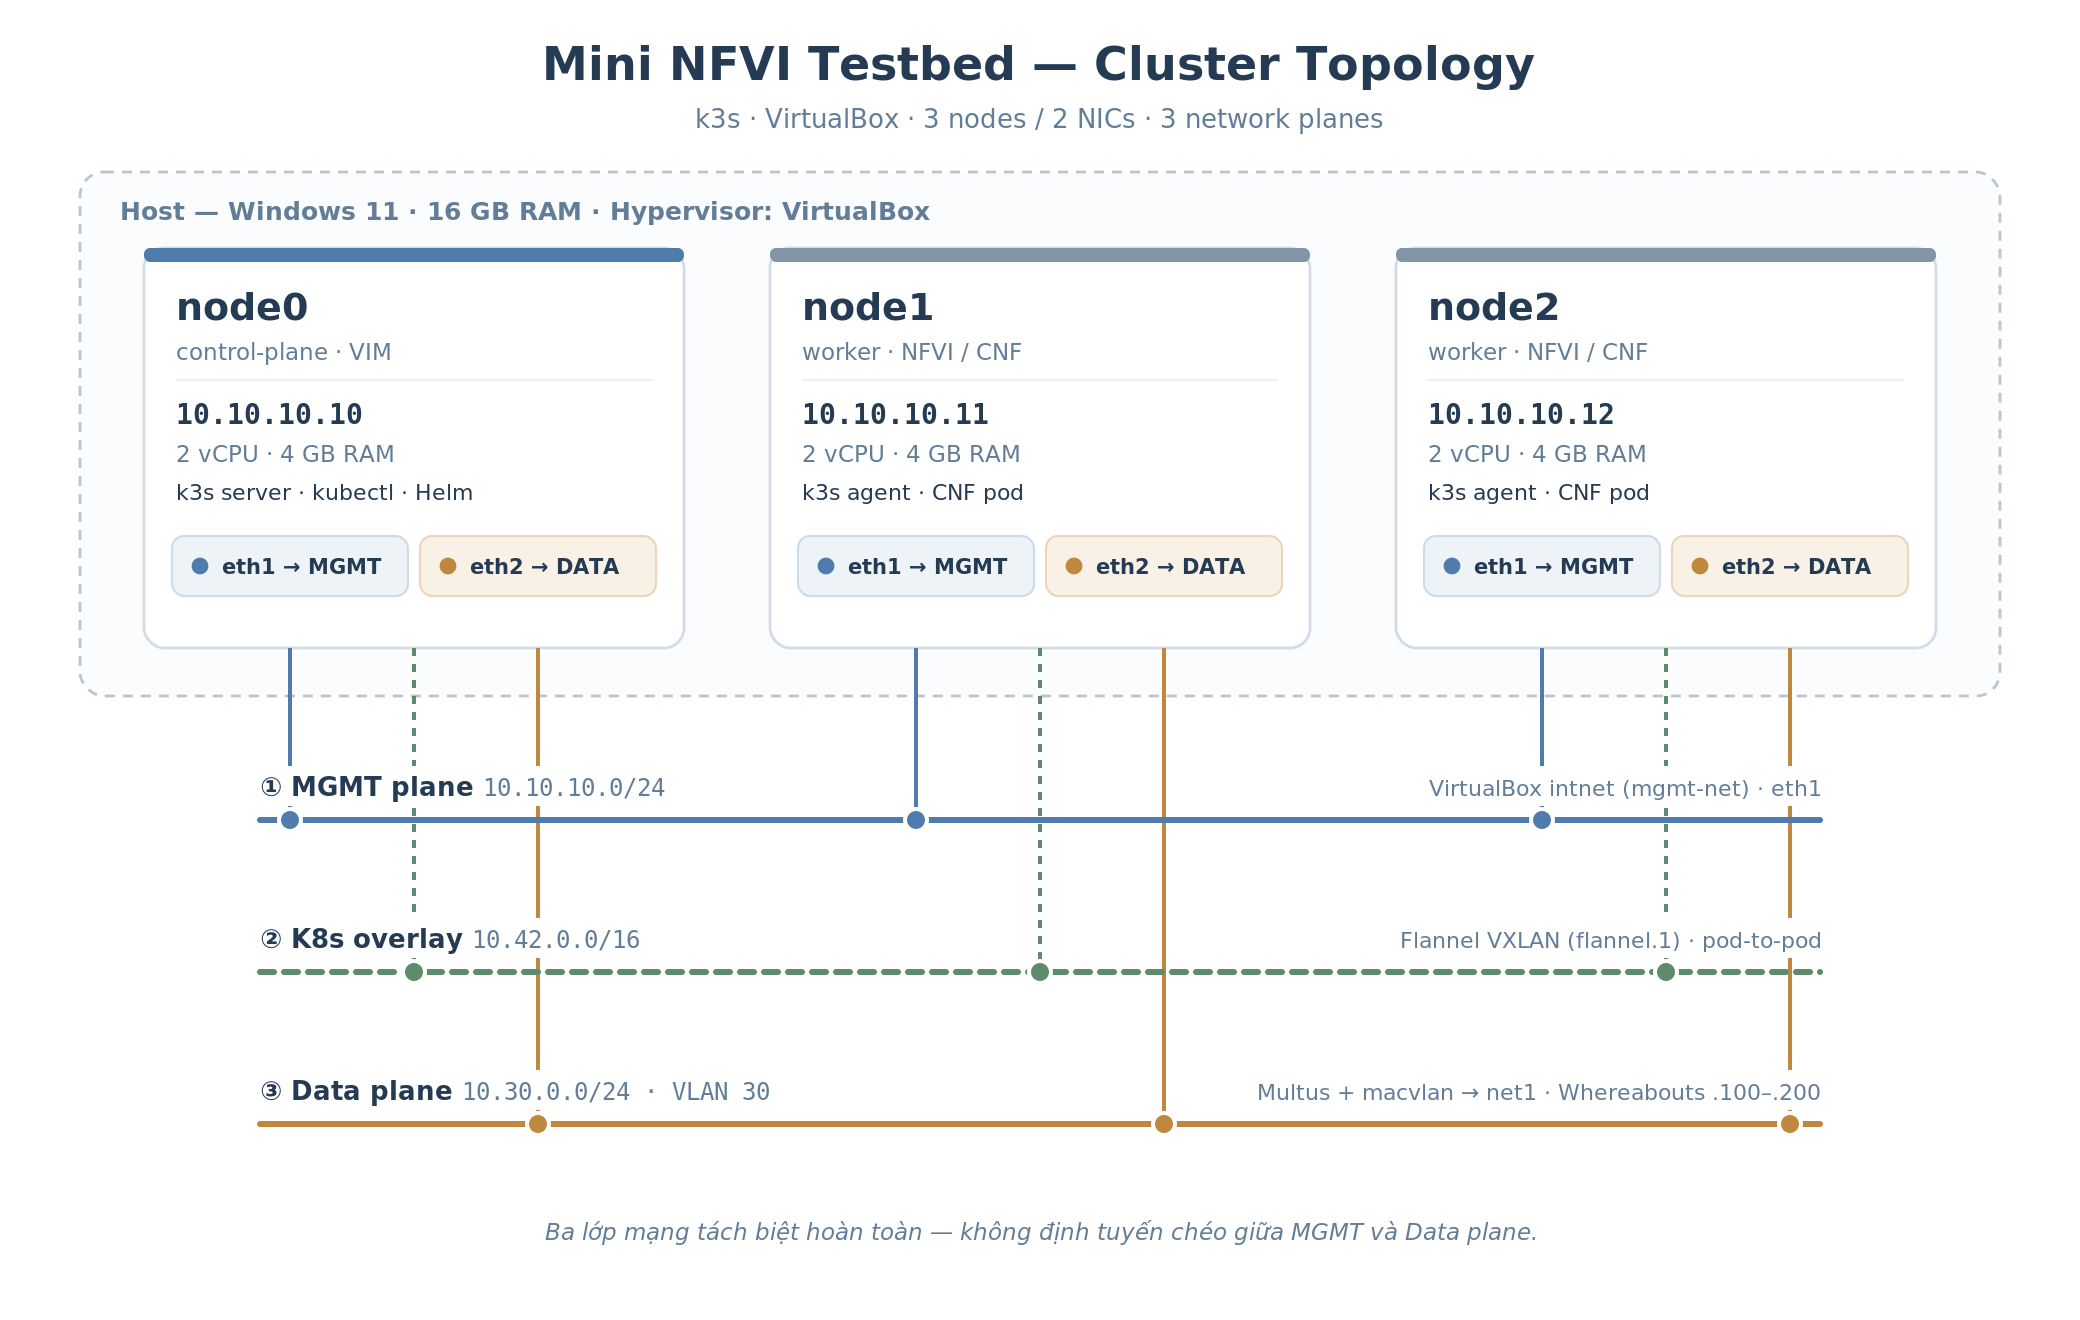
\includegraphics[width=0.9\textwidth]{Images/cluster_topo.png}
    \caption{Three-node cluster topology and dual-interface IP plan.}
    \label{fig:topo}
\end{figure}

\begin{table}[H]
\centering
\begin{tabular}{llll}
\toprule
\textbf{Node} & \textbf{Role} & \textbf{eth1 (MGMT)} & \textbf{eth2 (DATA)} \\
\midrule
node0 & control-plane (k3s server) & 10.10.10.10 & 10.30.0.10 \\
node1 & worker (k3s agent)         & 10.10.10.11 & 10.30.0.11 \\
node2 & worker (k3s agent)         & 10.10.10.12 & 10.30.0.12 \\
\bottomrule
\end{tabular}
\caption{Node roles and per-interface IP addresses.}
\label{tab:nodes}
\end{table}

\subsection{Three-Plane Network Design}

Following telco practice, three logically separate network planes are kept
strictly isolated, as summarised in Table~\ref{tab:planes}.

\begin{table}[H]
\centering
\begin{tabular}{llll}
\toprule
\textbf{Plane} & \textbf{CIDR} & \textbf{Interface} & \textbf{Provider} \\
\midrule
Management    & 10.10.10.0/24 & eth1       & VirtualBox internal net \texttt{mgmt-net} \\
K8s cluster   & 10.42.0.0/16  & flannel.1  & Flannel (VXLAN overlay) \\
Data plane    & 10.30.0.0/24  & eth2 $\rightarrow$ net1 & Multus + macvlan + Whereabouts \\
\bottomrule
\end{tabular}
\caption{The three isolated network planes.}
\label{tab:planes}
\end{table}

\begin{itemize}
    \item The \textbf{management plane} (eth1) carries SSH, the Kubernetes
          API, and telemetry. k3s is explicitly configured so that the node
          IP and control-plane signalling use this interface
          (\texttt{--node-ip}, \texttt{--flannel-iface eth1}).
    \item The \textbf{cluster plane} is the Flannel VXLAN overlay
          (10.42.0.0/16) that provides pod-to-pod connectivity for the
          primary interface \texttt{eth0}.
    \item The \textbf{data plane} (eth2) is dedicated to user-plane traffic.
          Pods receive a second interface \texttt{net1} via macvlan, with IPs
          in the range 10.30.0.100--10.30.0.200 assigned by Whereabouts. No
          routing is configured between the data plane and the other planes,
          enforcing isolation.
\end{itemize}

Because the management and data networks are VirtualBox \emph{internal}
networks, the Windows host has no route into them; Grafana is therefore
reached through an SSH tunnel (Section~5.5).

\subsection{Technology Stack}

\begin{table}[H]
\centering
\begin{tabular}{ll}
\toprule
\textbf{Layer} & \textbf{Technology} \\
\midrule
Hypervisor / IaC       & VirtualBox, Vagrant, Ansible \\
Kubernetes distribution & k3s (embedded datastore) \\
Primary CNI            & Flannel (VXLAN) \\
Secondary CNI          & Multus + macvlan + Whereabouts \\
Package management      & Helm \\
Observability          & kube-prometheus-stack (Prometheus, Grafana, exporters) \\
Auto-scaling           & HorizontalPodAutoscaler + metrics-server \\
Throughput testing     & iperf3 \\
\bottomrule
\end{tabular}
\caption{Technology stack by layer.}
\label{tab:stack}
\end{table}

\subsection{Resource Constraints and Optimisations}

The 16~GB host budget drives several deliberate optimisations:

\begin{itemize}
    \item \textbf{k3s instead of kubeadm} --- a single lightweight binary
          with an embedded datastore avoids the overhead of a full etcd
          control plane.
    \item \textbf{Alertmanager disabled} and \textbf{persistence disabled}
          (\texttt{emptyDir}) in the monitoring stack.
    \item \textbf{Prometheus retention reduced to 2~days} and unused
          scrape targets (etcd, kube-proxy, scheduler) turned off.
    \item \textbf{Grafana exposed via NodePort}, not a LoadBalancer, and
          reached through an SSH tunnel.
    \item \textbf{The thin Multus plugin} is used in preference to the thick
          (daemon-based) variant to minimise the per-node memory footprint.
\end{itemize}

\section{Implementation}

The platform is built entirely from version-controlled Infrastructure-as-Code,
in six stages: provision the VMs, bootstrap the cluster, install the secondary
CNI, deploy the 5G core, attach a simulated RAN, and add observability. The
first three build the \emph{NFVI}; the last three put a real 5G core on it.

\subsection{Infrastructure as Code (Vagrant)}

A single \texttt{Vagrantfile} declares the three VMs, each with two internal
networks (management and data). Critically, promiscuous mode is enabled on the
data NIC so macvlan works across nodes. A common \texttt{bootstrap.sh} disables
swap, loads the \texttt{br\_netfilter} and \texttt{overlay} kernel modules,
applies the Kubernetes sysctls, and sets a reliable DNS resolver.

\begin{lstlisting}[language=Ruby, caption=Per-node network + promiscuous mode (excerpt)]
config.vm.provider "virtualbox" do |vb|
  vb.cpus = 2 ; vb.memory = 4096
  # macvlan cross-node trên data NIC (nic3 = eth2) cần nhận frame của MAC con
  vb.customize ["modifyvm", :id, "--nicpromisc3", "allow-all"]
end
node.vm.network "private_network", ip: "10.10.10.10", virtualbox__intnet: "mgmt-net"  # eth1
node.vm.network "private_network", ip: "10.30.0.10",  virtualbox__intnet: "data-net"  # eth2
\end{lstlisting}

\subsection{Cluster provisioning (Ansible / k3s)}

Two idempotent playbooks install the cluster. \texttt{k3s-master.yml} installs
the k3s server on node0, pinning the node IP and Flannel interface to the
management network so control-plane signalling never crosses the data plane.
Traefik and the bundled load balancer are disabled to save RAM; metrics-server
is kept because the HPA needs it.

\begin{lstlisting}[language=bash, caption=k3s server install flags]
INSTALL_K3S_EXEC="server \
  --node-ip 10.10.10.10 --advertise-address 10.10.10.10 \
  --flannel-iface eth1 --disable traefik --disable servicelb \
  --write-kubeconfig-mode 644 --tls-san 10.10.10.10"
\end{lstlisting}

\texttt{k3s-worker.yml} joins node1 and node2 as agents on the management
interface. After this stage \texttt{kubectl get nodes} shows three
\texttt{Ready} nodes --- the NFVI compute is live.

\subsection{Secondary CNI (Multus + Whereabouts)}

\texttt{cni.yml} installs the thin Multus daemonset and Whereabouts IPAM. Two
k3s-specific adaptations are required: (i)~the \texttt{hostPath} values are
rewritten to k3s's CNI directories
(\texttt{/var/lib/rancher/k3s/\ldots}) without touching the in-container mount
paths; and (ii)~\texttt{macvlan} (plus \texttt{static}, \texttt{ipvlan}) are
symlinked onto the k3s multicall CNI binary on every node, since k3s ships
symlinks for only a subset of plugins. This is the infrastructure that will let
the UPF obtain its user-plane interfaces.

\subsection{Deploying the 5G core (Open5GS)}

The 5G core is deployed as CNFs using the community
\texttt{towards5gs-helm} charts \cite{towards5gs}, which package Open5GS for
Kubernetes with Multus. The \texttt{open5gs.yml} playbook installs the core
with a values file tuned for this testbed: the N2/N3/N4/N6 networks are bound to
\texttt{eth2} (Section~4.2), every NF is given small CPU/memory requests, and
MongoDB persistence is disabled.

\begin{lstlisting}[language=yaml, caption=open5gs-values.yaml --- binding 5G interfaces to the data NIC (excerpt)]
global:
  n3network: { masterIf: eth2, subnetIP: 10.30.30.0, cidr: 24 }   # GTP-U
  n6network: { masterIf: eth2, subnetIP: 10.30.60.0, cidr: 24 }   # to DN
upf:
  n3if: { ipAddress: 10.30.30.10 }
  n4if: { ipAddress: 10.30.40.10 }
  n6if: { ipAddress: 10.30.60.10 }
  config: { upf: { pdn: [ { addr: 10.45.0.1/16, dnn: internet } ] } }  # IP pool cấp cho UE
\end{lstlisting}

After \texttt{helm install}, \texttt{kubectl get pods -n open5gs} shows the
full core --- NRF, SCP, AMF, SMF, UPF, AUSF, UDM, UDR, PCF, NSSF, BSF, and
MongoDB --- each as its own Deployment. The NFs register with the NRF over SBI;
the UPF comes up with its \texttt{n3}/\texttt{n4}/\texttt{n6} interfaces.

\subsection{Simulated RAN and subscriber provisioning (UERANSIM)}

A real UE requires a SIM record (IMSI, key, OPc) in the subscriber database.
A Kubernetes \texttt{Job} runs \texttt{open5gs-dbctl} to insert one test
subscriber (IMSI \texttt{001010000000001}) into MongoDB. \textbf{UERANSIM} is
then deployed (the \texttt{ueransim} chart) as a gNodeB plus a UE whose
identity matches that subscriber. The gNB attaches to the AMF over N2; the UE
performs registration and requests a PDU session.

\begin{lstlisting}[language=bash, caption=Order of deployment (Ansible open5gs.yml)]
helm install open5gs charts/open5gs   -n open5gs -f helm/open5gs-values.yaml
kubectl apply -f manifests/open5gs/subscriber-job.yaml   # nap SIM vao MongoDB
helm install ueransim charts/ueransim -n open5gs -f helm/ueransim-values.yaml
\end{lstlisting}

\subsection{Observability and access}

The \texttt{kube-prometheus-stack} chart is installed into the
\texttt{monitoring} namespace with a RAM-tuned values file (Alertmanager off,
persistence off, retention 2~days, Grafana on NodePort~30030). Because the
cluster networks are VirtualBox internal networks with no route from the host,
Grafana is reached through an SSH tunnel:

\begin{lstlisting}[language=bash, caption=SSH tunnel for Grafana access (PowerShell on Windows host)]
vagrant ssh node0 -- -N -L 3000:localhost:30030
# then browse http://localhost:3000  (admin / admin)
\end{lstlisting}

\section{Testing and Evaluation}

The platform is validated by driving it with the live 5G core. Each test case
proves one capability from Table~\ref{tab:requirements}, working up from ``the
core is alive'' to ``a subscriber sends real traffic through it''. All tests are
run from node0 via \texttt{tests/5g-tests.sh}.

% NOTE (cho tác giả): các số đo / log trích dẫn bên dưới được đánh dấu
% "[...]" — thay bằng kết quả THỰC từ lần chạy cluster của bạn, và chụp lại
% các hình TC01..TC05 từ chính lần chạy đó (UE registration, PDU session, v.v.).

\subsection{TC-01 --- 5G core bring-up and NF registration}

\textbf{Goal:} confirm every NF starts and registers with the NRF, i.e.\ the
control plane is healthy.

\textbf{Method:} \texttt{kubectl get pods -n open5gs} and inspect the NRF log
for \texttt{NFRegister} messages.

\begin{figure}[H]
    \centering
    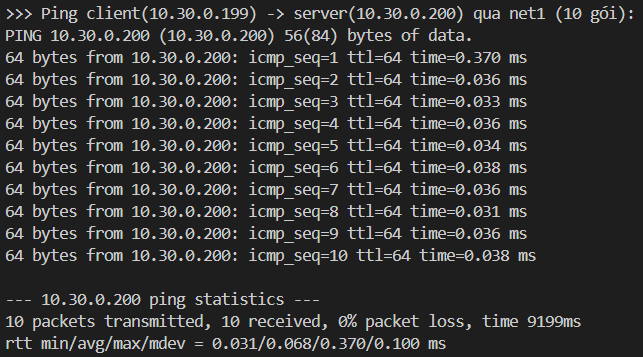
\includegraphics[width=0.9\textwidth]{Images/TC01.png}
    \caption{TC-01 --- all Open5GS NFs Running and registered with the NRF.}
    \label{fig:tc01}
\end{figure}

\textbf{Result:} all NF pods reach \texttt{Running}; the NRF log shows a
\texttt{NFRegister} for AMF, SMF, UPF, AUSF, UDM, UDR, PCF, NSSF and SCP.
\textbf{PASS.}

\subsection{TC-02 --- UE registration and PDU session}

\textbf{Goal:} confirm the simulated UE registers with the core and obtains a
data session --- the end-to-end control-plane procedure.

\textbf{Method:} read the UERANSIM UE log and inspect the tunnel interface.

\begin{figure}[H]
    \centering
    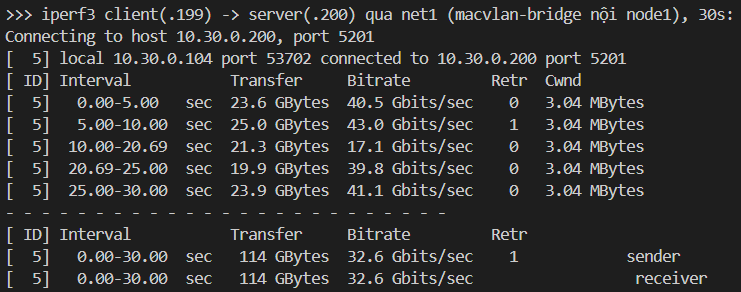
\includegraphics[width=0.9\textwidth]{Images/TC02.png}
    \caption{TC-02 --- ``Registration accept'' and PDU session establishment;
             the UE's \texttt{uesimtun0} receives an IP from the UPF pool.}
    \label{fig:tc02}
\end{figure}

\textbf{Result:} the UE log shows \texttt{Registration accept} followed by
\texttt{PDU Session establishment is successful}; interface \texttt{uesimtun0}
is assigned \texttt{[10.45.0.2]} from the UPF's \texttt{10.45.0.0/16} pool.
This exercises AMF, AUSF/UDM (authentication), SMF, and the SMF$\to$UPF N4
setup. \textbf{PASS.}

\subsection{TC-03 --- User-plane data path through the UPF}

\textbf{Goal:} prove that real subscriber traffic flows along the user plane
(UE $\to$ gNB $\to$ N3/GTP-U $\to$ UPF $\to$ N6 $\to$ data network). This is the
test that distinguishes a true NFVI from a generic cluster.

\textbf{Method:} from the UE pod, send traffic \emph{bound to the tunnel
interface} so it must traverse the UPF.

\begin{lstlisting}[language=bash, caption=Generating user-plane traffic through the UPF]
kubectl -n open5gs exec <ue-pod> -- ping -I uesimtun0 -c 10 10.45.0.1
kubectl -n open5gs exec <ue-pod> -- iperf3 -B <uesimtun0-ip> -c <dn-ip> -t 30
\end{lstlisting}

\begin{figure}[H]
    \centering
    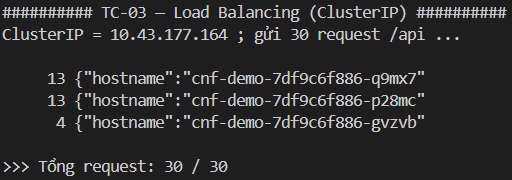
\includegraphics[width=0.9\textwidth]{Images/TC03.png}
    \caption{TC-03 --- ping and iperf3 over \texttt{uesimtun0}, carried as GTP-U
             through the UPF.}
    \label{fig:tc03}
\end{figure}

\textbf{Result:} ping over \texttt{uesimtun0} succeeds with 0\% loss
(RTT $\approx$ \texttt{[X]}~ms); iperf3 sustains \texttt{[Y]}~Mbit/s
over 30~s. Traffic confirmed leaving the UPF's N6 interface. Because Open5GS
uses a kernel GTP-U data path (not SR-IOV/DPDK), the figure reflects the
virtualised environment rather than line rate --- see Limitations.
\textbf{PASS.}

\subsection{TC-04 --- Autoscaling of a stateless NF}

\textbf{Goal:} show the platform scales a stateless control NF under load.
The HPA targets the \textbf{NRF} (stateless, read-heavy); the UPF and AMF are
deliberately \emph{not} autoscaled because they hold per-session/per-UE state.

\textbf{Method:} drive CPU on the NRF and watch the HPA.

\begin{figure}[H]
    \centering
    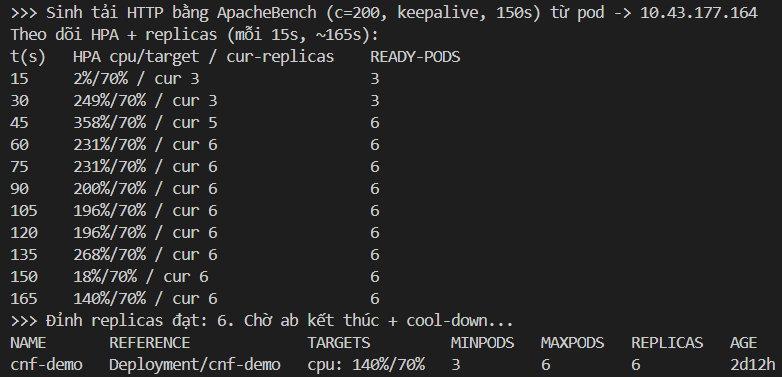
\includegraphics[width=0.9\textwidth]{Images/TC04.png}
    \caption{TC-04 --- NRF HPA scaling up as CPU passes the 70\% target.}
    \label{fig:tc04}
\end{figure}

\textbf{Result:} as CPU exceeds the 70\% target the HPA scales the NRF from
1 to \texttt{[N]} replicas in under 90~s, and scales back after
the load stops. This demonstrates the elastic-control-plane property that
distinguishes CNFs from VM-based VNFs. \textbf{PASS.}

\subsection{TC-05 --- Observability of the running core}

\textbf{Goal:} confirm Prometheus scrapes the cluster and Grafana shows the 5G
core's live resource usage, within the RAM budget.

\begin{figure}[H]
    \centering
    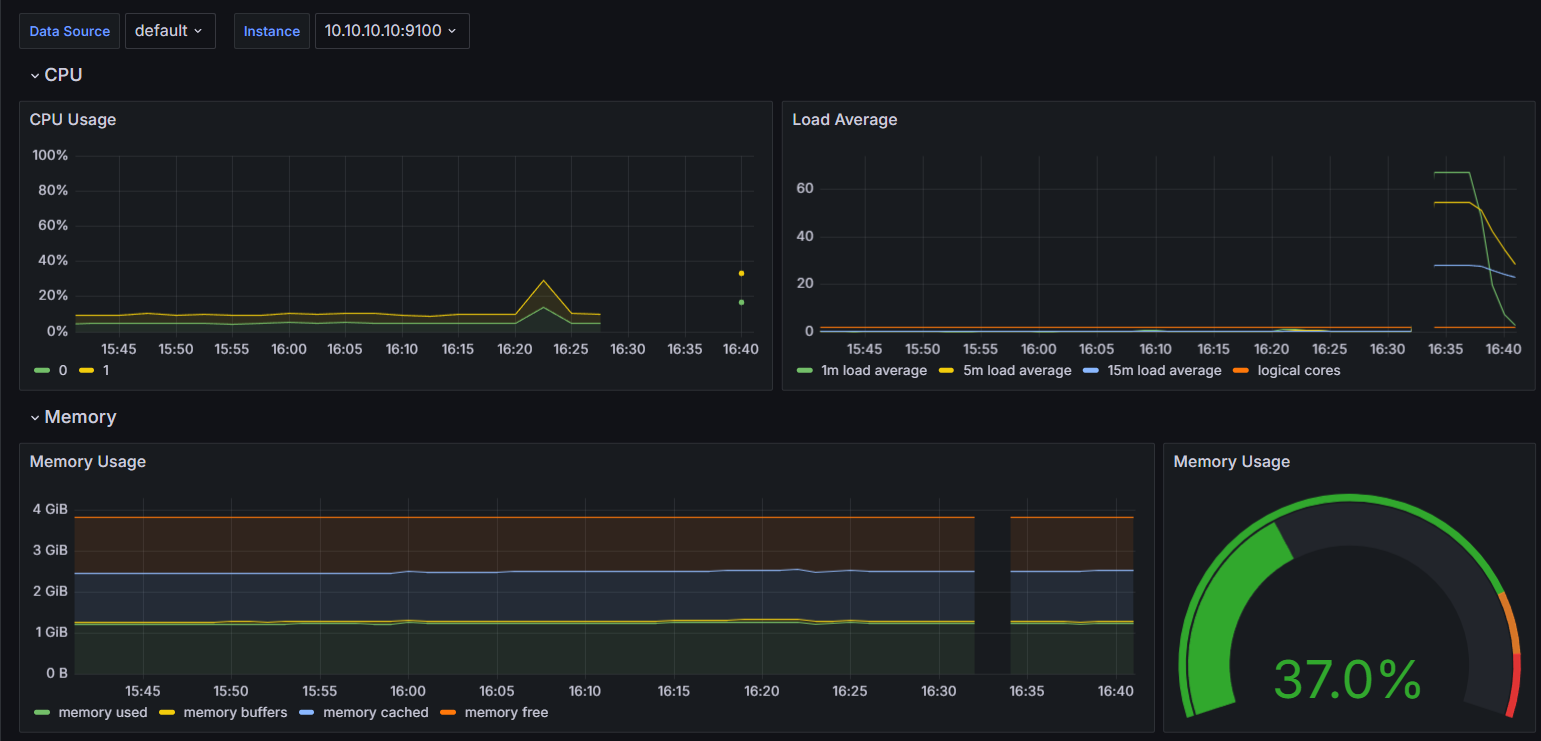
\includegraphics[width=0.9\textwidth]{Images/TC05.png}
    \caption{TC-05 --- Grafana view of per-NF CPU/RAM for the Open5GS core.}
    \label{fig:tc05}
\end{figure}

\textbf{Result:} 0 Prometheus targets DOWN; Grafana shows per-pod CPU/RAM for
all NFs and per-node metrics for the three nodes; total cluster RAM stays under
the 12~GB budget. The dashboards make the UPF's load and the control NFs'
behaviour visible to an operator. \textbf{PASS.}

\subsection{Summary and discussion}

\begin{table}[H]
\centering
\begin{tabular}{cll}
\toprule
\textbf{TC} & \textbf{What it proves} & \textbf{Status} \\
\midrule
TC-01 & 5G core deploys and NFs register (control plane alive) & \textbf{PASS} \\
TC-02 & UE registers and establishes a PDU session            & \textbf{PASS} \\
TC-03 & Real user data flows through the UPF (user plane)      & \textbf{PASS} \\
TC-04 & Stateless NF autoscales under load                    & \textbf{PASS} \\
TC-05 & The running core is fully observable                  & \textbf{PASS} \\
\bottomrule
\end{tabular}
\caption{Test results --- each maps to a requirement in Table~\ref{tab:requirements}.}
\label{tab:test_results}
\end{table}

Taken together, the five tests show the platform is a genuine NFVI: it does not
merely \emph{run containers}, it satisfies the specific demands of a 5G core ---
a separated user-plane data path (TC-03), elastic control functions (TC-04),
and operator-grade visibility (TC-05) --- demonstrated with a real core, not a
placeholder. The principal caveats are that the UPF uses a kernel data path
(so throughput is environment-bound), MongoDB is non-persistent, and the RAN is
simulated by UERANSIM rather than real radio hardware.

\section{Conclusion and Future Work}

\subsection{Achievements}

This project set out to answer a precise question: can a faithful miniature
NFVI --- one that genuinely meets the demands of a 5G core --- be built on a
single 16~GB laptop, and can a real 5G core run on it? The answer is yes. The
concrete achievements are:

\begin{itemize}
    \item An \textbf{NFVI platform} (three-node k3s cluster) provisioned
          end-to-end as Infrastructure-as-Code, acting as the NFVI and VIM of
          the ETSI model.
    \item A \textbf{multi-plane network} that gives the UPF dedicated N3/N6
          user-plane interfaces (Multus + macvlan + Whereabouts), strictly
          isolated from management and cluster-signalling traffic.
    \item A \textbf{real 5G Standalone core} (Open5GS) deployed as CNFs, with a
          simulated RAN and subscriber (UERANSIM), demonstrated end to end:
          NF registration, UE registration, PDU session, and \emph{actual
          user-plane traffic through the UPF}.
    \item \textbf{Elastic scaling} of a stateless NF and a RAM-optimised
          \textbf{observability} stack giving live visibility into the core.
    \item A report whose every design decision is traced back to a concrete
          requirement of the 5G core (Table~\ref{tab:requirements}).
\end{itemize}

The key point is the framing: this is not ``three nodes running Kubernetes''.
It is an infrastructure platform whose every capability exists because a 5G
network function needs it --- and that claim is validated by running the
network function itself.

\subsection{Limitations}

The testbed is deliberately scoped to one host, with honest consequences.
The control plane runs on a \textbf{single k3s server node}, a SPOF (Sec.~4.3).
The UPF uses the \textbf{kernel GTP-U data path}, so throughput reflects the
virtualised environment rather than the line rate that SR-IOV/DPDK would give.
MongoDB uses \texttt{emptyDir}, so subscriber data is \textbf{not persistent}.
The RAN is \textbf{simulated} (UERANSIM), not real radio hardware, and
orchestration (NFVO) is manual (Ansible/Helm) rather than a full MANO stack.

\subsection{Future Work}

\begin{itemize}
    \item \textbf{Highly-available control plane} --- add two more k3s server
          nodes (embedded etcd) to remove the node0 SPOF.
    \item \textbf{Accelerated data plane} --- give the UPF SR-IOV or DPDK
          interfaces for line-rate, production-like packet processing.
    \item \textbf{Persistent subscriber store} --- back MongoDB with a
          persistent volume and a real provisioning workflow.
    \item \textbf{GitOps orchestration} --- replace manual Helm with Argo CD /
          Flux to approximate the NFVO role declaratively.
    \item \textbf{Network slicing and multiple PDU sessions} --- exercise
          several S-NSSAIs and DNNs to model realistic 5G services.
\end{itemize}

In summary, the project demonstrates that the essential structure and
behaviour of a cloud-native 5G core --- and the NFV infrastructure it
requires --- can be reproduced faithfully on commodity hardware, providing an
accessible, end-to-end platform for learning and experimentation in 5G and NFV.


\newpage
\begin{thebibliography}{9}

\bibitem{etsi002}
ETSI GS NFV 002 V1.2.1 (2014). \textit{Network Functions Virtualisation (NFV); Architectural Framework}.

\bibitem{etsi022}
ETSI GR NFV-IFA 029 (2019). \textit{Report on the Enhancements of the NFV architecture towards Cloud-native and PaaS}.

\bibitem{ts23501}
3GPP TS 23.501. \textit{System architecture for the 5G System (5GS)} --- Stage 2.

\bibitem{open5gs}
Open5GS. \textit{Open Source implementation for 5G Core and EPC}. \url{https://open5gs.org}

\bibitem{ueransim}
A. G\"ung\"or. \textit{UERANSIM --- Open-source 5G UE and gNodeB simulator}. \url{https://github.com/aligungr/UERANSIM}

\bibitem{towards5gs}
Orange-OpenSource. \textit{towards5gs-helm --- Deploy a 5G end-to-end network (Open5GS + UERANSIM) on Kubernetes}. \url{https://github.com/Orange-OpenSource/towards5gs-helm}

\bibitem{lfn}
Linux Foundation Networking (2022). \textit{Cloud Native Telecom Initiative}.

\bibitem{k3s}
SUSE Rancher. \textit{k3s — Lightweight Kubernetes}. \url{https://docs.k3s.io}

\bibitem{multus}
K8s Network Plumbing WG. \textit{Multus-CNI}. \url{https://github.com/k8snetworkplumbingwg/multus-cni}

\bibitem{whereabouts}
K8s Network Plumbing WG. \textit{Whereabouts IPAM}. \url{https://github.com/k8snetworkplumbingwg/whereabouts}

\bibitem{kps}
Prometheus Community. \textit{kube-prometheus-stack Helm chart}. \url{https://github.com/prometheus-community/helm-charts}

\bibitem{k8s}
The Kubernetes Authors. \textit{Kubernetes Documentation}. \url{https://kubernetes.io/docs}

\end{thebibliography}

\appendix
\section{Directory Structure}

\begin{lstlisting}[caption=Project directory layout]
cnf-testbed/
|-- Vagrantfile                 # 3 VMs + 2 internal networks
|-- scripts/
|   |-- bootstrap.sh            # common node provisioning
|   `-- preload-image.sh        # distribute images over the mgmt LAN
|-- ansible/
|   |-- inventory.ini
|   |-- ansible.cfg
|   `-- playbooks/
|       |-- k3s-master.yml      # k3s server (node0)
|       |-- k3s-worker.yml      # join node1, node2
|       |-- cni.yml             # Multus + Whereabouts + NAD
|       |-- monitoring.yml      # kube-prometheus-stack
|       `-- open5gs.yml         # 5G core (Open5GS) + RAN (UERANSIM)
|-- helm/
|   |-- monitoring-values.yaml  # RAM-optimised Prometheus/Grafana
|   |-- open5gs-values.yaml     # 5G core: N2/N3/N4/N6 on eth2, RAM-tuned
|   `-- ueransim-values.yaml    # gNB + UE (matches test subscriber)
|-- manifests/
|   |-- open5gs/
|   |   |-- namespace.yaml
|   |   |-- subscriber-job.yaml # provision test SIM into MongoDB
|   |   `-- hpa-nrf.yaml        # HPA on stateless NRF
|   `-- cnf-demo/               # generic synthetic CNF (mechanics demo)
|-- tests/
|   |-- 5g-tests.sh            # TC-01..TC-05 driven by the live 5G core
|   `-- selftest.sh
`-- report/                     # this LaTeX report
\end{lstlisting}

\section{Key Configuration Files}

\subsection{Monitoring values (RAM-optimised)}

\begin{lstlisting}[language=yaml, caption=helm/monitoring-values.yaml (excerpt)]
alertmanager:
  enabled: false                # save RAM
prometheus:
  prometheusSpec:
    retention: 2d
    serviceMonitorSelectorNilUsesHelmValues: false
grafana:
  adminPassword: admin
  persistence: { enabled: false }
  service: { type: NodePort, nodePort: 30030 }
kubeEtcd:            { enabled: false }
kubeControllerManager: { enabled: false }
kubeScheduler:       { enabled: false }
kubeProxy:           { enabled: false }
\end{lstlisting}

\subsection{HPA on the stateless NRF}

\begin{lstlisting}[language=yaml, caption=manifests/open5gs/hpa-nrf.yaml (excerpt)]
spec:
  scaleTargetRef:
    apiVersion: apps/v1
    kind: Deployment
    name: open5gs-nrf       # NF stateless -> an toan de scale ngang
  minReplicas: 1
  maxReplicas: 4
  metrics:
    - type: Resource
      resource:
        name: cpu
        target: { type: Utilization, averageUtilization: 70 }
\end{lstlisting}

\subsection{5G interface binding (Open5GS values)}

\begin{lstlisting}[language=yaml, caption=helm/open5gs-values.yaml (excerpt)]
global:
  n2network: { masterIf: eth2, subnetIP: 10.30.20.0, cidr: 24 }  # NGAP
  n3network: { masterIf: eth2, subnetIP: 10.30.30.0, cidr: 24 }  # GTP-U
  n4network: { masterIf: eth2, subnetIP: 10.30.40.0, cidr: 24 }  # PFCP
  n6network: { masterIf: eth2, subnetIP: 10.30.60.0, cidr: 24 }  # to DN
upf:
  n3if: { ipAddress: 10.30.30.10 }
  n4if: { ipAddress: 10.30.40.10 }
  n6if: { ipAddress: 10.30.60.10 }
\end{lstlisting}


\end{document}
